%\documentclass[aps,prd,preprint]{revtex4-1}
\documentclass[aps,prd,final,twocolumn,floats,floatfix,nofootinbib,10pt]{revtex4-1}

% Note:  comment out one of the two documentclass commands, depending
% on whether you need the final or preprint version. It is most convenient
% to work in preprint mode, and switch to final only at the end.

\usepackage{graphicx}
\usepackage{amsmath}
\usepackage{amsfonts}
\usepackage{amssymb}
\usepackage{amstext}
\usepackage[english]{babel}
\usepackage{helvet}
\usepackage{microtype}
\usepackage{dsfont}
\usepackage[pdftex]{hyperref}
\usepackage{tikz}

\special{papersize=8.5in,11in}
\setlength{\pdfpageheight}{\paperheight}
\setlength{\pdfpagewidth}{\paperwidth}

\usetikzlibrary{calc,decorations.markings}

\begin{document}


\title{Deriving Green's function for d'Alembert operator}
\author{indutny}
\date{\today}
\noaffiliation

\begin{abstract}
Green's functions play vital role in all physical disciplines. Most sophisticated Quantum Field Theory and
General Relativity calculations would rely on knowing Green's function for computing general solutions. In fact
obtaining the Green's function for an operator is equivalent to obtaining the operator's inverse. In this short and
terse paper we obtain the Green's function for a d'Alembert operator ``$\square$".
\end{abstract}

\maketitle

\section{Overview}

\subsection{Conventions}

It is common in General Relativity texts to use following convention for the metric:
\begin{equation}
\eta_{\mu\nu} = \eta^{\mu\nu} = \begin{pmatrix}
-1 & 0 & 0 & 0 \\
0 & 1 & 0 & 0 \\
0 & 0 & 1 & 0 \\
0 & 0 & 0 & 1
\end{pmatrix}.
\end{equation}
With this metric in mind the d'Alembert operator becomes:
\begin{equation}
\square f(x) = \eta^{\mu\nu} \partial_\mu \partial_\nu f(x) =
  \left( -\partial_0 \partial_0 + \partial_i \partial^i \right) f(x),
\end{equation}
where repeated latin or greek indices are assumed to be summed as per Einstein's convention.

We will denote 4-vectors as $p$ and 3-vector part of it as $\vec{p}$. The norm of both is $|p|$ and $|\vec{p}|$
respectively.

The normalization for Fourier transforms is chosen such that:
\begin{align}
\tilde{f}(p) & = \int d^4x \; e^{-i p \cdot x } f(x), \\
f(x) & = \int \frac{d^4p}{(2 \pi)^4} e^{i p \cdot x} \tilde{f}(p).
\end{align}

Heaviside step function $\Theta(x)$ is $1$ for $x > 0$ and $0$ otherwise.

\subsection{Green's function}

Our goal is to solve:
\begin{equation}\label{eq:dalembert-eq}
\square \Psi(x - y) = \eta^{\mu\nu} \partial_\mu \partial_\nu \Psi(x - y) = \delta^{(4)} (x - y)
\end{equation}
for $\Psi(x - y)$ (Note that $\partial_\mu$ here is $\frac{\partial}{\partial x^\mu}$).
The resulting function can be used to compute the solutions to more general differential equation:
\begin{equation}\label{eq:general-eq}
\square h(x) = T(x).
\end{equation}
Given the $\Psi(x - y)$ the reader can check that the solution to \eqref{eq:general-eq} is:
\begin{equation}
h(x) = \int d^4y \; \Psi(x - y) T(y).
\end{equation}

We wanted to be as explicit as possible in our solution. Thus it is our hope that the reader would forgive us the
excessive amount of steps.

\section{Solution}

\subsection{Initial Steps}

First of all, instead of solving for $\Psi(x - y)$ we could solve for $\Psi(x)$ and then shift the argument of the function
to get the end result. Substituting the Fourier transforms
\begin{align}\label{eq:fourier-transform}
\Psi(x) & = \int \frac{d^4p}{(2 \pi)^4} e^{i p \cdot x} \tilde{\Psi}(p) \\
\delta^{(4)} (x) & = \int \frac{d^4p}{(2 \pi)^4} e^{i p \cdot x} \cdot 1
\end{align}
into \eqref{eq:dalembert-eq} we get:
\begin{align}\label{eq:fourier-step}
\int \frac{d^4p}{(2 \pi)^4} e^{i p \cdot x} \left[ \eta^{\mu\nu} (-i p_\mu) (-i p_\nu) \tilde{\Psi}(p) - 1 \right] & = \\
\int \frac{d^4p}{(2 \pi)^4} e^{i p \cdot x} \left[ -p^2 \tilde{\Psi}(p) - 1 \right] & = 0.
\end{align}
Thus
\begin{equation}\label{eq:fourier-solution}
\tilde{\Psi}(p) = -\frac{1}{p^2}
\end{equation}
should in general solve \eqref{eq:fourier-step}. Plugging \eqref{eq:fourier-solution} back into
\eqref{eq:fourier-transform} we see that
\begin{equation}\label{eq:complex-integral}
\Psi(x) = \int \frac{d^4p}{(2 \pi)^4} e^{i p \cdot x} \frac{1}{p^2}.
\end{equation}

Going to spherical coordinates for $\vec{p}$ and separating $p_0$ we get following integral:
\begin{align}\label{eq:expanded-integral}
& \int_0^{2 \pi} \frac{d \phi}{2 \pi} \int_{-1}^{1} \frac{d \cos{\theta}}{2 \pi} \int \frac{d |\vec{p}|}{2 \pi}
  \int \frac{d p_0}{2 \pi} |\vec{p}|^2 e^{i p \cdot x} \left( \cdots \right) = \\
& \; \; \frac{1}{4 \pi^2} \int_{-1}^{1} d \cos{\theta} \int d |\vec{p}|
  \int \frac{d p_0}{2 \pi} e^{i p \cdot x} |\vec{p}|^2 \left( \cdots \right)
\end{align}
and
\begin{align}
e^{i p \cdot x} & = e^{-i p_0 t + i |x| |\vec{p}| \cos{\theta}}, \\
\left( \cdots \right) & = \frac{1}{p^2} = -\frac{1}{(p_0)^2 - |\vec{p}|^2}.
\end{align}

\subsection{Time component}

Let's look at $p_0$ part of the integral first:
\begin{equation}\label{eq:time-initial}
-\int \frac{d p_0}{2 \pi} e^{-i p_0 t} \frac{1}{(p_0)^2 - |\vec{p}|^2}.
\end{equation}
This integral can be solved in the complex plane if we shift the denominator slightly from the real axis (or equivalently shift the integration variable). Note that despite looking peculiar this is a perfectly valid trick in Complex Analysis. In fact this trick is ubiquitous in physics! With this in mind \eqref{eq:time-initial} becomes:
\begin{align}
& -\lim_{\epsilon \to 0} \int \frac{d p_0}{2 \pi} e^{-i p_0 t} \frac{1}{(p_0)^2 - |\vec{p}|^2 \mp i \epsilon} = \\
& -\lim_{\epsilon \to 0} \int \frac{d p_0}{2 \pi} e^{-i p_0 t} \frac{1}{p_0 + \left( |\vec{p}| \pm i \epsilon \right)}
  \frac{1}{p_0 - \left(|\vec{p}| \pm i \epsilon \right)} \label{eq:expanded-time}.
\end{align}

For each sign of $\pm i \epsilon$ we have two different poles and the integration contour can be closed
\textbf{below} when $t > 0$:
\begin{center}
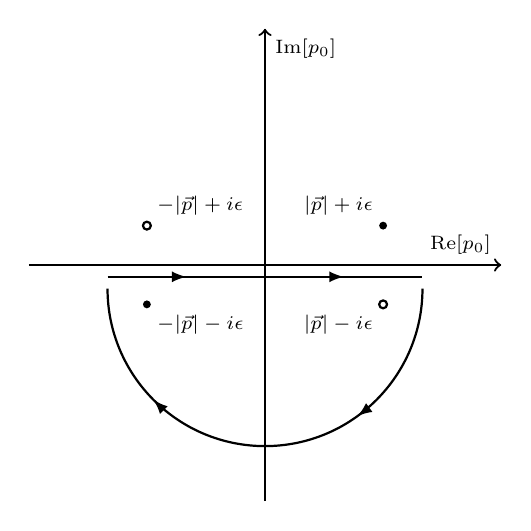
\begin{tikzpicture}
\begin{scope}[thick,font=\scriptsize]
% Axes:
\draw [->] (-3,0) -- (3,0) node [above left]  {$\text{Re}[p_0]$};
\draw [->] (0,-3) -- (0,3) node [below right] {$\text{Im}[p_0]$};

% Poles
\path [draw=none, fill=black] (1.5, 0.5) circle (0.05);
\node [above left, black] at (1.5, 0.5) {$|\vec{p}| + i \epsilon$};

\path [draw=none, fill=black] (-1.5, -0.5) circle (0.05);
\node [below right, black] at (-1.5, -0.5) {$-|\vec{p}| - i \epsilon$};

\path [draw=black, fill=none] (1.5, -0.5) circle (0.05);
\node [below left, black] at (1.5, -0.5) {$|\vec{p}| - i \epsilon$};

\path [draw=black, fill=none] (-1.5, 0.5) circle (0.05);
\node [above right, black] at (-1.5, 0.5) {$-|\vec{p}| + i \epsilon$};

% Contours

\draw[thick,decoration={ markings,
      mark=at position 0.25 with {\arrow{latex}}, 
      mark=at position 0.75 with {\arrow{latex}}}, 
      postaction={decorate}]
 (-2,-0.15) -- (2,-0.15);
\draw[thick,decoration={ markings,
      mark=at position 0.3 with {\arrow{latex}}, 
      mark=at position 0.75 with {\arrow{latex}}}, 
      postaction={decorate}]
 (2,-0.3) arc (0:-180:2);

\end{scope}
\end{tikzpicture}
\end{center}
(Note that we drew the bottom part of the contour disjoint from the rest to emphasize that it can be added
to the integral without changing the value of \eqref{eq:expanded-time} because $e^{-i p_0 t}$ becomes
infinitesimal at $\text{Im}[p_0] \to -\infty$. Adding this curve lets us close the contour and use the Residue
theorem.)

The integration contour picks either of the poles in the bottom half of the complex plane and we get:
\begin{equation}\label{eq:time-solution-ret}
t > 0 : \eqref{eq:expanded-time} = \mp i \lim_{\epsilon \to 0} \frac{1}{2 |\vec{p}| \pm i \epsilon}
  e^{\pm i \left(|\vec{p}| \pm i \epsilon\right) t}.
\end{equation}

Similar solution for $t < 0$ and with contour closed above (the reader can check the behavior of
$e^{i p_0 t}$ for negative $t$ and $p_0$ far on the positive imaginary axis) is:
\begin{equation}\label{eq:time-solution-adv}
t < 0 : \eqref{eq:expanded-time} = \mp i \lim_{\epsilon \to 0} \frac{1}{2 |\vec{p}| \pm i \epsilon}
  e^{\mp i \left(|\vec{p}| \pm i \epsilon\right) t}.
\end{equation}

\end{document}